\section{Kiến trúc hệ thống và Pipeline}
\label{sec:system-pipeline}

\subsection{Kiến trúc tổng thể hệ thống NewsLens}

Hệ thống \textbf{NewsLens} được xây dựng theo mô hình kiến trúc phân tầng module hóa (layered modular architecture), tách bạch giữa tầng giao diện người dùng (Presentation Layer), tầng dịch vụ và điều phối (Application Service Layer), và tầng lõi nghiệp vụ RAG (Core RAG Engine). Toàn bộ mã nguồn, cấu hình triển khai và hướng dẫn thiết lập hệ thống được lưu trữ công khai tại kho lưu trữ GitHub của đồ án: \url{https://github.com/ThomasdeCarpio/Text-Mining---NewsQA-RAG/tree/main}. Thiết kế này vừa phục vụ tương tác hỏi đáp thời gian thực cho người dùng cuối, vừa đóng vai trò như một nền tảng phục vụ công tác nghiên cứu và giám sát thực nghiệm.

\subsubsection{Tầng giao diện người dùng (Frontend Client)}
Được xây dựng bằng React và TypeScript, cung cấp hai giao diện tương tác chính:
\begin{itemize}
  \item \textbf{Màn hình Hỏi đáp (Chat Interface):} Giao diện đối thoại cho phép người dùng nhập câu hỏi và nhận câu trả lời kèm danh sách trích dẫn nguồn (\texttt{CitationList}). Người dùng có thể nhấp chọn ``View Sources'' để xem chi tiết trích đoạn văn bản gốc, tiêu đề bài báo, ngày xuất bản và liên kết URL tới bài báo nguồn CNN.
  \item \textbf{Bàn thử nghiệm Truy xuất (Retrieval Playground):} Màn hình phục vụ kiểm thử độc lập tầng truy xuất. Người dùng có thể kiểm tra dung lượng bộ chỉ mục, nhập truy vấn tùy ý, lựa chọn giữa các thuật toán truy xuất (Dense, BM25, Sparse BGE-M3, Hybrid, hoặc Locked), tùy biến tham số Top-$k$, và theo dõi điểm tương đồng cùng biểu đồ phân rã độ trễ của từng thành phần (bộ truy xuất hay bộ tái xếp hạng).
\end{itemize}

\subsubsection{Tầng dịch vụ điều phối (Backend Application Services)}
Được hiện thực bằng FastAPI trên nền Python, chịu trách nhiệm quản lý phiên làm việc, phân luồng yêu cầu và kết nối giao diện với tầng lõi RAG:
\begin{itemize}
  \item \texttt{chat\_service.py}: Quản lý phiên hội thoại, điều phối tiến trình gọi pipeline RAG và phản hồi câu trả lời kèm trích dẫn nguồn cho người dùng.
  \item \texttt{retrieval\_service.py}: Thực hiện các truy vấn tìm kiếm trực tiếp vào kho chỉ mục vector hoặc chỉ mục thưa theo yêu cầu từ giao diện.
  \item \texttt{auth\_service.py}: Xác thực phiên làm việc cho người dùng và khách truy cập trong môi trường trình diễn đồ án.
\end{itemize}

\subsubsection{Tầng lõi RAG dùng chung (\texttt{common/newsqa\_rag})}
Được tổ chức thành thư viện Python độc lập (\texttt{newsqa\_rag}) có thể tái sử dụng nhất quán giữa ứng dụng web, các tập lệnh CLI (\texttt{scripts/}) và notebook nghiên cứu:
\begin{itemize}
  \item \textbf{Module nạp và phân đoạn văn bản (\texttt{ingestion/}):} Tiền xử lý văn bản thô, làm sạch ký tự và chia tách bài báo thành các đoạn (chunks) theo các chiến lược: Recursive Character Splitter (kích thước và độ chồng lặp tùy biến), Sentence Splitter, Paragraph Splitter và Phân cấp Parent--Child.
  \item \textbf{Module lập chỉ mục (\texttt{indexing/}):} Quản lý cơ sở dữ liệu vector Chroma (\texttt{ChromaDB}) lưu trữ dense embeddings từ các mô hình như BGE-M3 \cite{chen2024bge} hoặc MiniLM \cite{reimers2019sentence}, đồng thời quản lý chỉ mục đảo thưa được tối ưu hóa bằng BM25S \cite{robertson2009probabilistic}.
  \item \textbf{Module truy xuất và tái xếp hạng (\texttt{retrieval/}):} Cung cấp các lớp giao tiếp cho Dense Retriever, Sparse Retriever, Hybrid Retriever (kết hợp điểm số theo Reciprocal Rank Fusion -- RRF \cite{cormack2009reciprocal}) và mô hình tái xếp hạng chéo Cross-Encoder (\texttt{bge-reranker-large} \cite{xiao2023c}).
  \item \textbf{Module tác tử và giao tiếp LLM (\texttt{agents/}, \texttt{llm.py}):} Hiện thực lớp điều phối \texttt{RAGAgent}, đóng gói các mẫu chỉ thị trong kho đăng ký prompt (P0--P3, B0--B2) và kết nối với các mô hình ngôn ngữ lớn (Gemini 3.1 Flash-Lite, GPT-4o-mini).
  \item \textbf{Module phân tích và đánh giá (\texttt{evaluation/}, \texttt{response\_parsing.py}):} Bóc tách nhãn trích dẫn \texttt{[n]}, ánh xạ về ID đoạn văn bản nguồn, kiểm tra tính hợp lệ của trích dẫn và kết nối bộ giám khảo RAGAS \cite{es2023ragas}.
\end{itemize}

\subsection{Quy trình xử lý Pipeline RAG End-to-End}

Khi tiếp nhận truy vấn, hệ thống NewsLens thực thi tuần tự quy trình 6 bước xử lý khép kín:

\begin{enumerate}
  \item \textbf{Bước 1: Tiếp nhận và xử lý câu hỏi (Query Ingestion):}
  Quy trình tiếp nhận được phân định rõ ràng theo hai trường hợp sử dụng (use cases):
  \begin{itemize}
    \item \textbf{Đối với ứng dụng Chat thực tế:} Hệ thống tiếp nhận trực tiếp câu hỏi tự nhiên từ người dùng qua API để chuyển thẳng vào luồng truy xuất và trả lời.
    \item \textbf{Đối với hệ thống đánh giá thực nghiệm (Benchmark):} Pipeline sử dụng tập câu hỏi đã được chuẩn hóa ngữ cảnh (Resolved Questions) từ bộ dữ liệu NewsQA ---
trong đó tên thực thể và mốc sự kiện đã được bổ sung đầy đủ --- nhằm đánh giá độc lập và khách quan năng lực định vị bằng chứng của các mô hình truy xuất trên kho dữ liệu
quy mô lớn.
  \end{itemize}  
  \item \textbf{Bước 2: Truy xuất ứng viên giai đoạn 1 (First-Stage Candidate Retrieval):}
  Bộ truy xuất thưa \textbf{BGE-M3 Sparse Retriever} quét kho \NumCorpusChunks{} đoạn văn bản (từ \NumCorpusArticles{} bài báo CNN) dựa trên trọng số từ vựng chuyên biệt, trích xuất tập hợp \NumPoneTopK{} đoạn ứng viên có điểm số cao nhất (thời gian xử lý $11\text{--}15\text{ ms}$).

  \item \textbf{Bước 3: Tái xếp hạng chéo giai đoạn 2 (Second-Stage Cross-Encoder Reranking):}
  Tập \NumPoneTopK{} đoạn ứng viên được đưa qua mô hình \textbf{BGE-Reranker-Large}. Mô hình Cross-Encoder đánh giá đồng thời cặp (Câu hỏi, Đoạn văn) qua cơ chế cross-attention của transformer để phân tích tương quan ngữ nghĩa sâu, chọn lọc ra \NumPoneRerankTopN{} đoạn văn bản liên quan nhất cung cấp cho bộ sinh.

  \item \textbf{Bước 4: Đóng gói ngữ cảnh và định dạng chỉ thị (Context Assembly \& Prompt Formatting):}
  Năm đoạn văn bản được định dạng theo danh sách đánh số \texttt{[1]} đến \texttt{[5]}, kết hợp cùng mẫu chỉ thị \textbf{Prompt P2}. Mẫu prompt này yêu cầu mô hình: (i) chỉ dựa vào thông tin có trong 5 đoạn văn bản; (ii) trả lời ngắn gọn, trực diện đúng loại thông tin được hỏi; và (iii) bắt buộc gắn nhãn trích dẫn \texttt{[n]} ngay sau mỗi sự kiện.

  \item \textbf{Bước 5: Sinh câu trả lời có kiểm chứng (Grounded Generation):}
  Ngữ cảnh và chỉ thị được gửi tới mô hình ngôn ngữ lớn \textbf{Gemini 3.1 Flash-Lite} (với \texttt{temperature = 0}, \texttt{reasoning = minimal}, giới hạn 512 tokens) để sinh câu trả lời có nguồn dẫn.

  \item \textbf{Bước 6: Bóc tách cú pháp và xác thực trích dẫn (Citation Validation):}
  Bộ phân tích \texttt{response\_parsing.py} quét chuỗi câu trả lời để bóc tách nhãn trích dẫn \texttt{[n]}, kiểm tra tính hợp lệ trong dải $\{1, \dots, 5\}$, và ánh xạ chỉ số này về Chunk ID cùng metadata bài báo gốc để hiển thị minh bạch cho người dùng.
\end{enumerate}

\subsection{Sơ đồ minh họa Pipeline}

Hình~\ref{fig:rag-pipeline} minh họa kiến trúc pipeline hai tầng của NewsLens từ khâu chuẩn bị dữ liệu offline đến luồng xử lý truy xuất và sinh câu trả lời online.

\begin{figure}[H]
  \centering
  \IfFileExists{../figures/pipeline.png}{%
    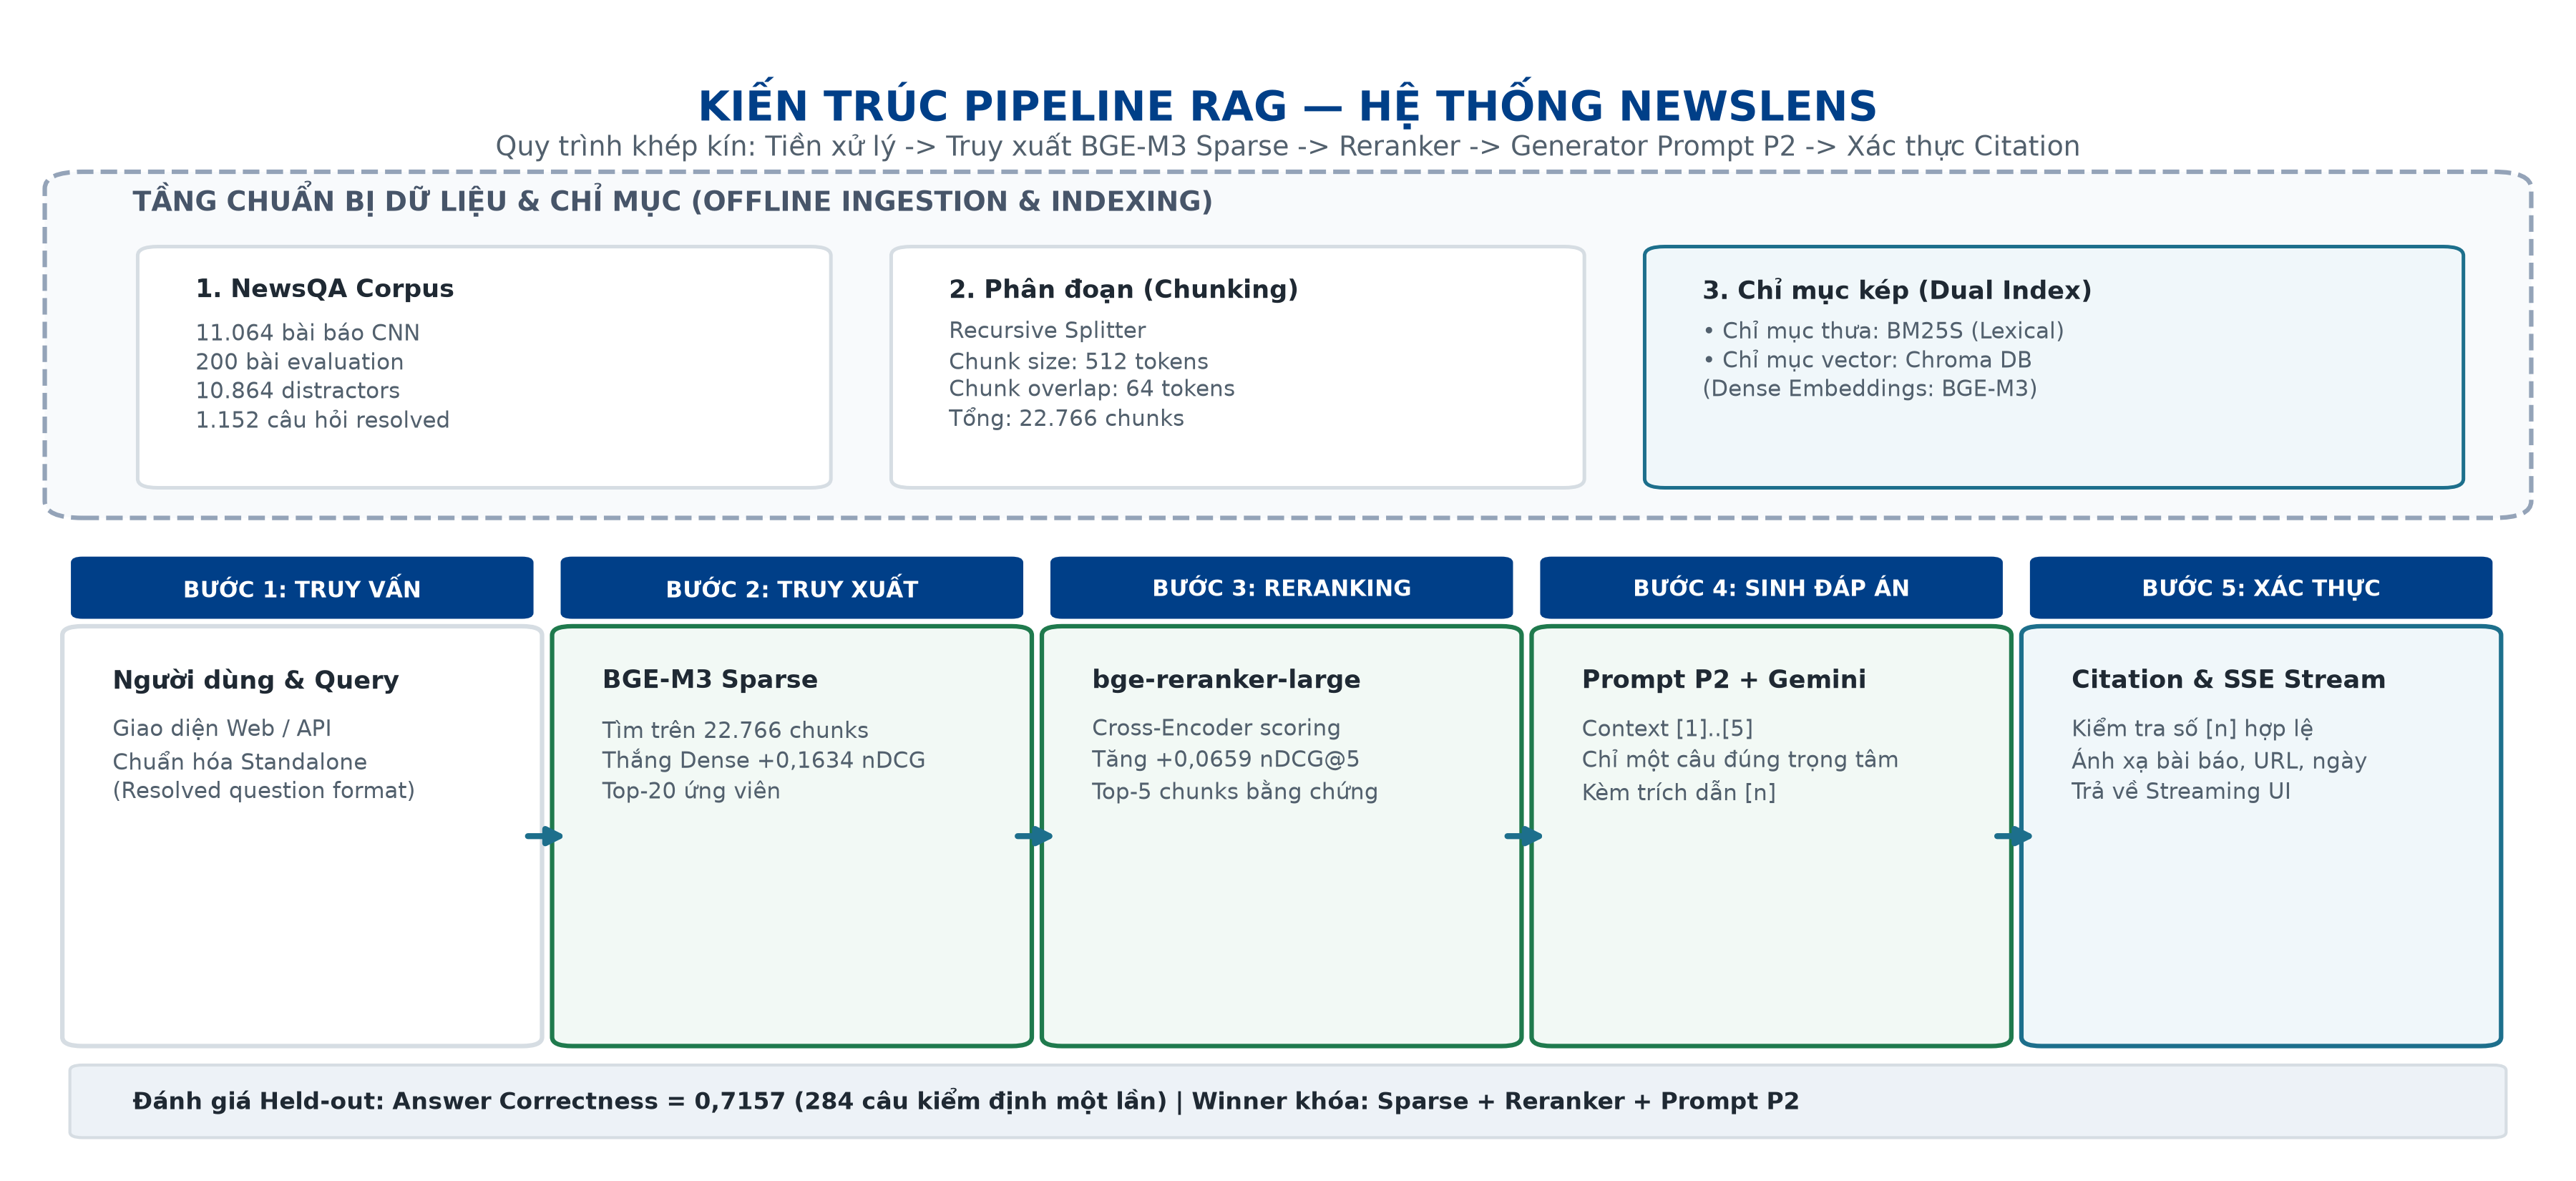
\includegraphics[width=\textwidth]{../figures/pipeline.png}%
  }{%
    \begin{center}
      \framebox[\textwidth]{\rule{0pt}{7cm}\textbf{[Hình: Sơ đồ Pipeline RAG NewsLens -- Vui lòng xuất từ figures/pipeline\_diagram.html và lưu thành figures/pipeline.png]}}
    \end{center}
  }
  \caption{Sơ đồ kiến trúc Pipeline RAG hai tầng của hệ thống NewsLens: Tầng Offline (Chuẩn bị dữ liệu NewsQA, phân đoạn văn bản 512/64 và lập chỉ mục kép) và Tầng Online (Truy xuất thưa BGE-M3 Top-20, Tái xếp hạng BGE-Reranker Top-5, Sinh đáp án với Prompt P2 trên Gemini 3.1 Flash-Lite, và Xác thực trích dẫn nguồn).}
  \label{fig:rag-pipeline}
\end{figure}

\noindent\textbf{Ghi chú mã nguồn sơ đồ:} Nhóm tác giả đã đóng gói sơ đồ kiến trúc này dưới dạng tệp tương tác HTML/CSS độc lập tại \path{docs/latex/figures/pipeline_diagram.html}, tích hợp mã nguồn Mermaid và bố cục trực quan độ nét cao.

\subsection{Giao diện người dùng và Minh họa ứng dụng}

Dưới đây là minh họa hai phân hệ người dùng chính của NewsLens đang hoạt động trên môi trường thực tế:

\subsubsection{Giao diện Hỏi đáp tin tức (News Chat)}
Hình~\ref{fig:app-chat} thể hiện màn hình đối thoại trực tiếp. Khi người dùng đặt câu hỏi (ví dụ vụ án Nithari), hệ thống kích hoạt pipeline, trả về câu trả lời \emph{``Pandher was sentenced to death in February 2009 [1].''} kèm thẻ trích dẫn \texttt{[1]}. Khi mở rộng mục \textbf{View Sources}, khung chi tiết sẽ hiển thị trích đoạn bài báo CNN gốc, ngày đăng, vị trí đoạn văn bản chứa bằng chứng và đường dẫn URL nguồn.

\begin{figure}[H]
  \centering
  \IfFileExists{../figures/chat_interface.png}{%
    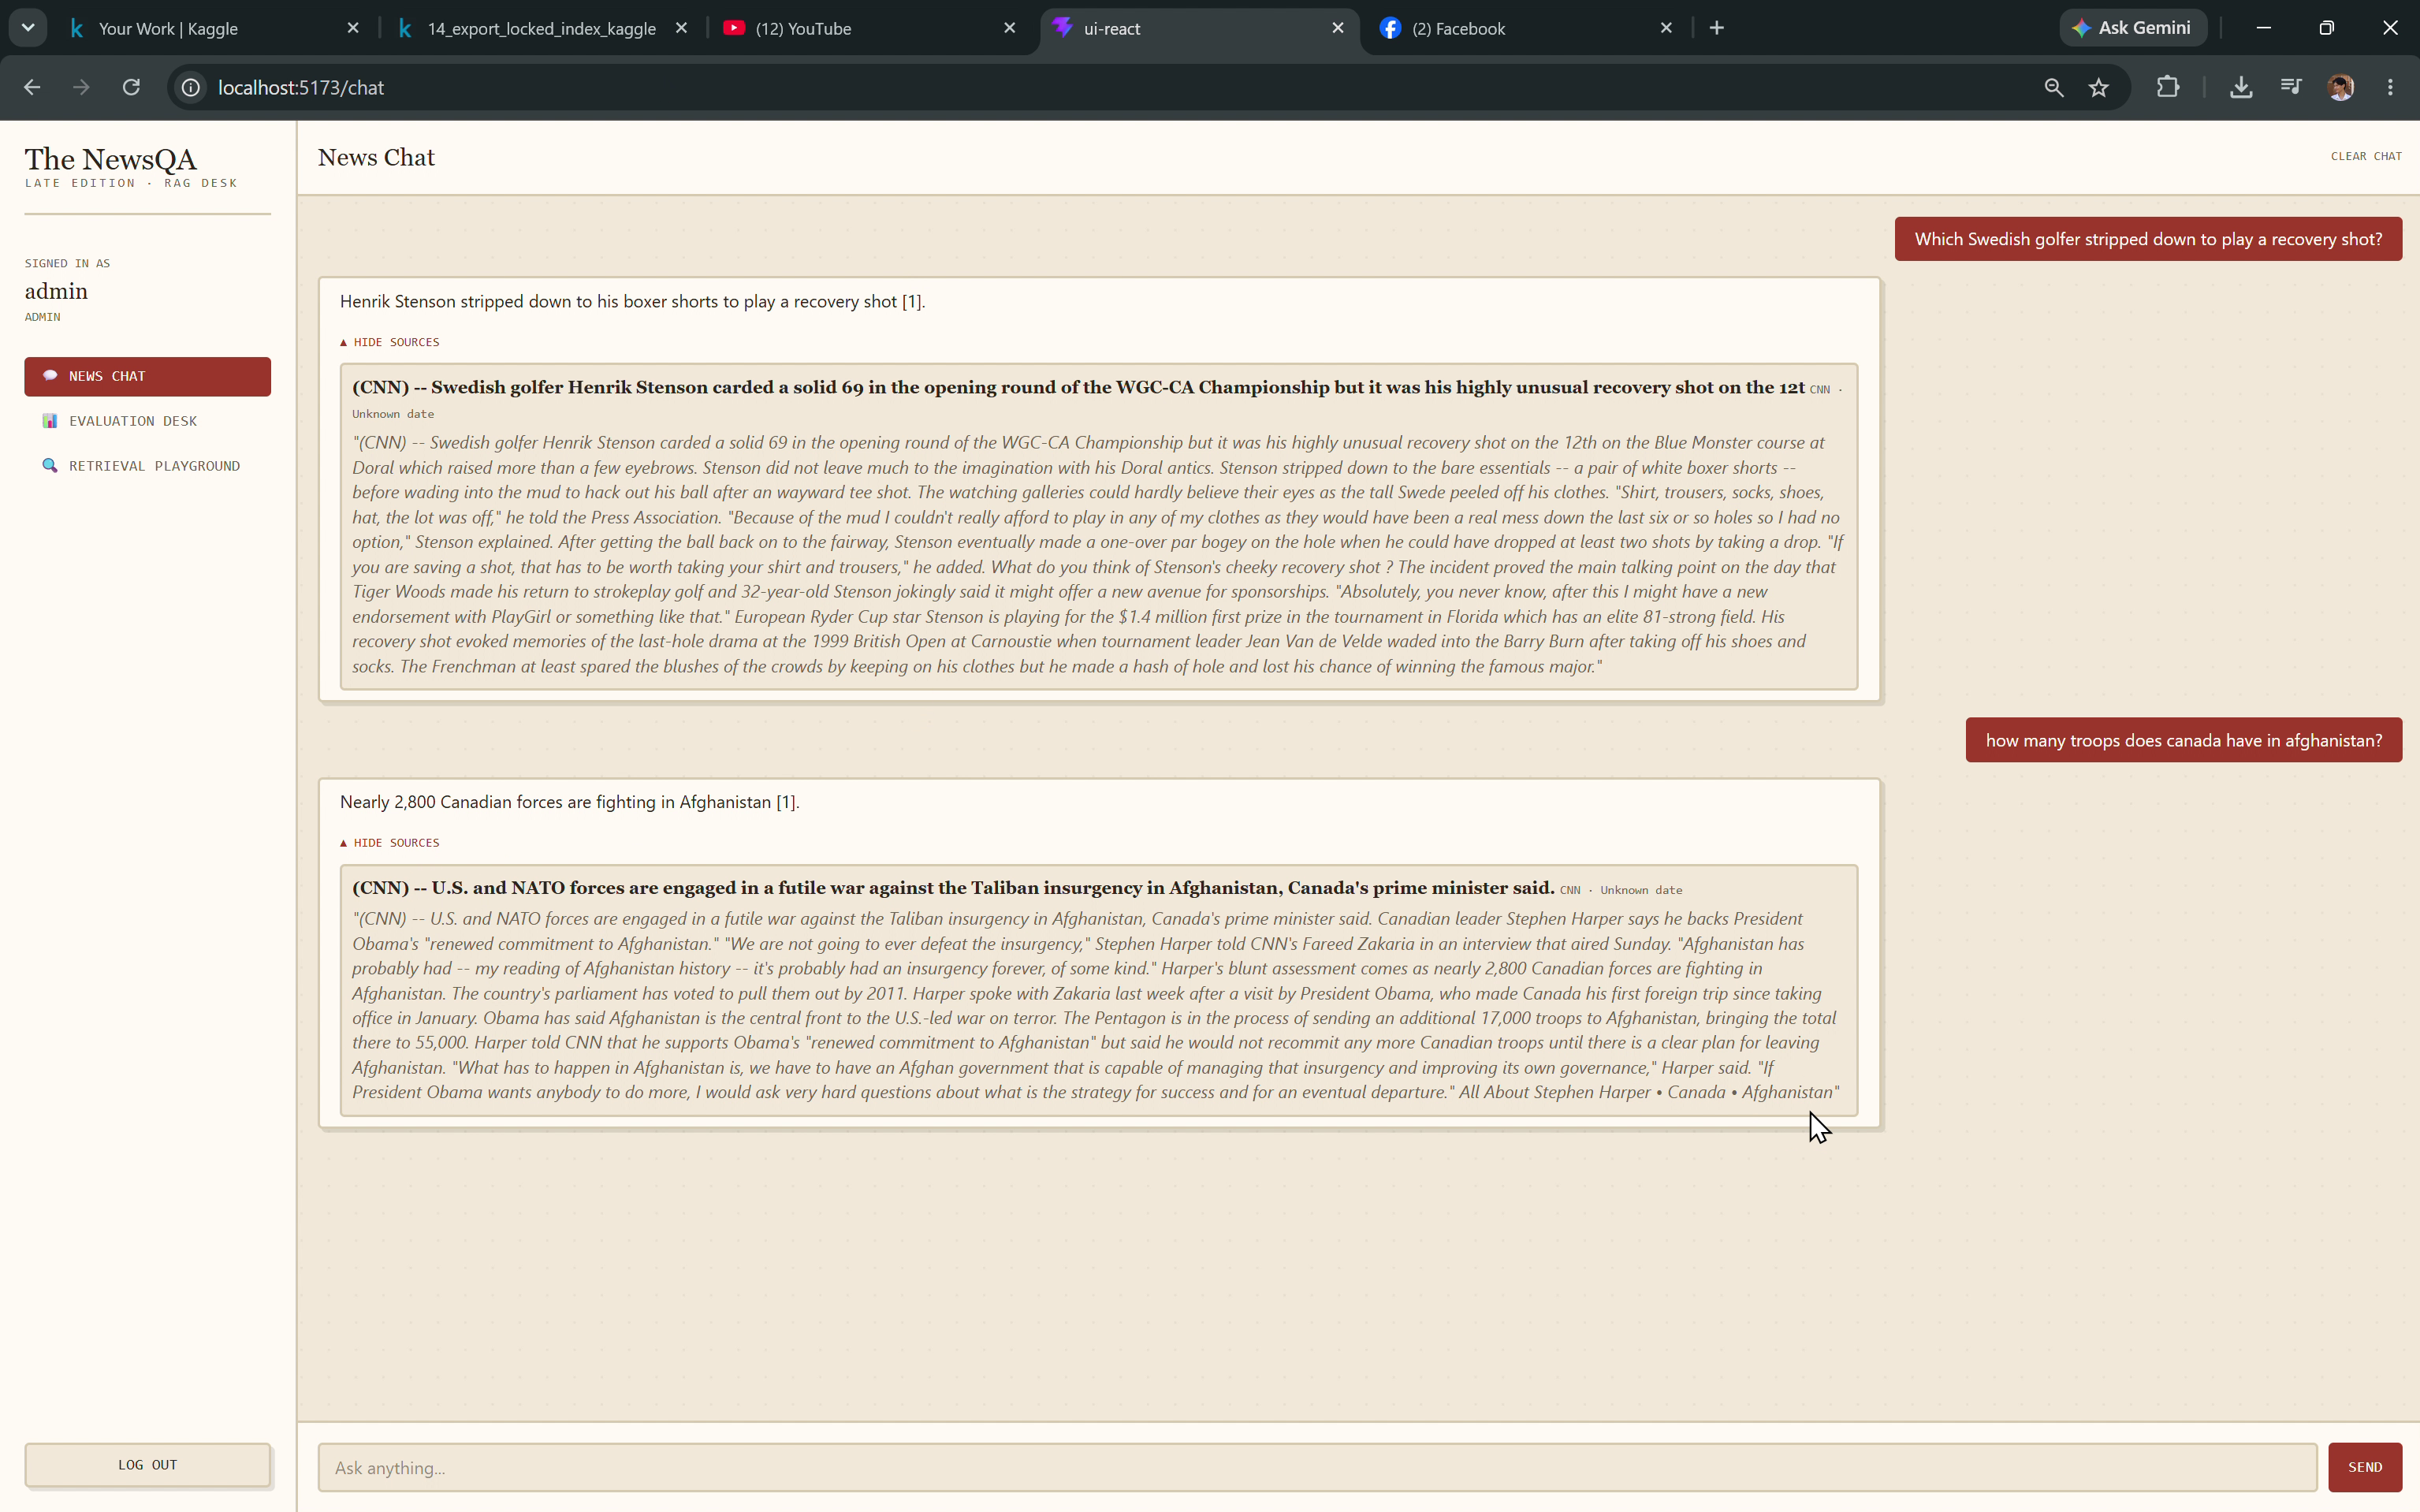
\includegraphics[width=0.92\textwidth]{../figures/chat_interface.png}%
  }{%
    \begin{center}
      \framebox[0.92\textwidth]{\rule{0pt}{6.5cm}\textbf{[Hình: Giao diện News Chat với trích dẫn tương tác và nguồn bằng chứng]}}
    \end{center}
  }
  \caption{Giao diện Hỏi đáp NewsLens (News Chat): Phản hồi câu trả lời súc tích kèm ký hiệu trích dẫn \texttt{[1]} và khung mở rộng ``View Sources'' hiển thị trích đoạn bài báo CNN cùng liên kết URL gốc.}
  \label{fig:app-chat}
\end{figure}

\subsubsection{Bàn thử nghiệm Truy xuất (Retrieval Playground)}
Hình~\ref{fig:app-retrieval} thể hiện công cụ kiểm thử tầng truy xuất độc lập. Người dùng có thể kiểm tra kho chỉ mục \NumCorpusChunks{} đoạn văn bản, nhập truy vấn kiểm thử, so sánh giữa các thuật toán truy xuất, xem điểm số tương đồng của từng đoạn văn ứng viên và phân tích biểu đồ độ trễ thực thi của từng bước (Sparse: $12\text{ ms}$, Reranker: $498\text{ ms}$, Tổng cộng: $510\text{ ms}$).

\begin{figure}[H]
  \centering
  \IfFileExists{../figures/retrieval_playground.png}{%
    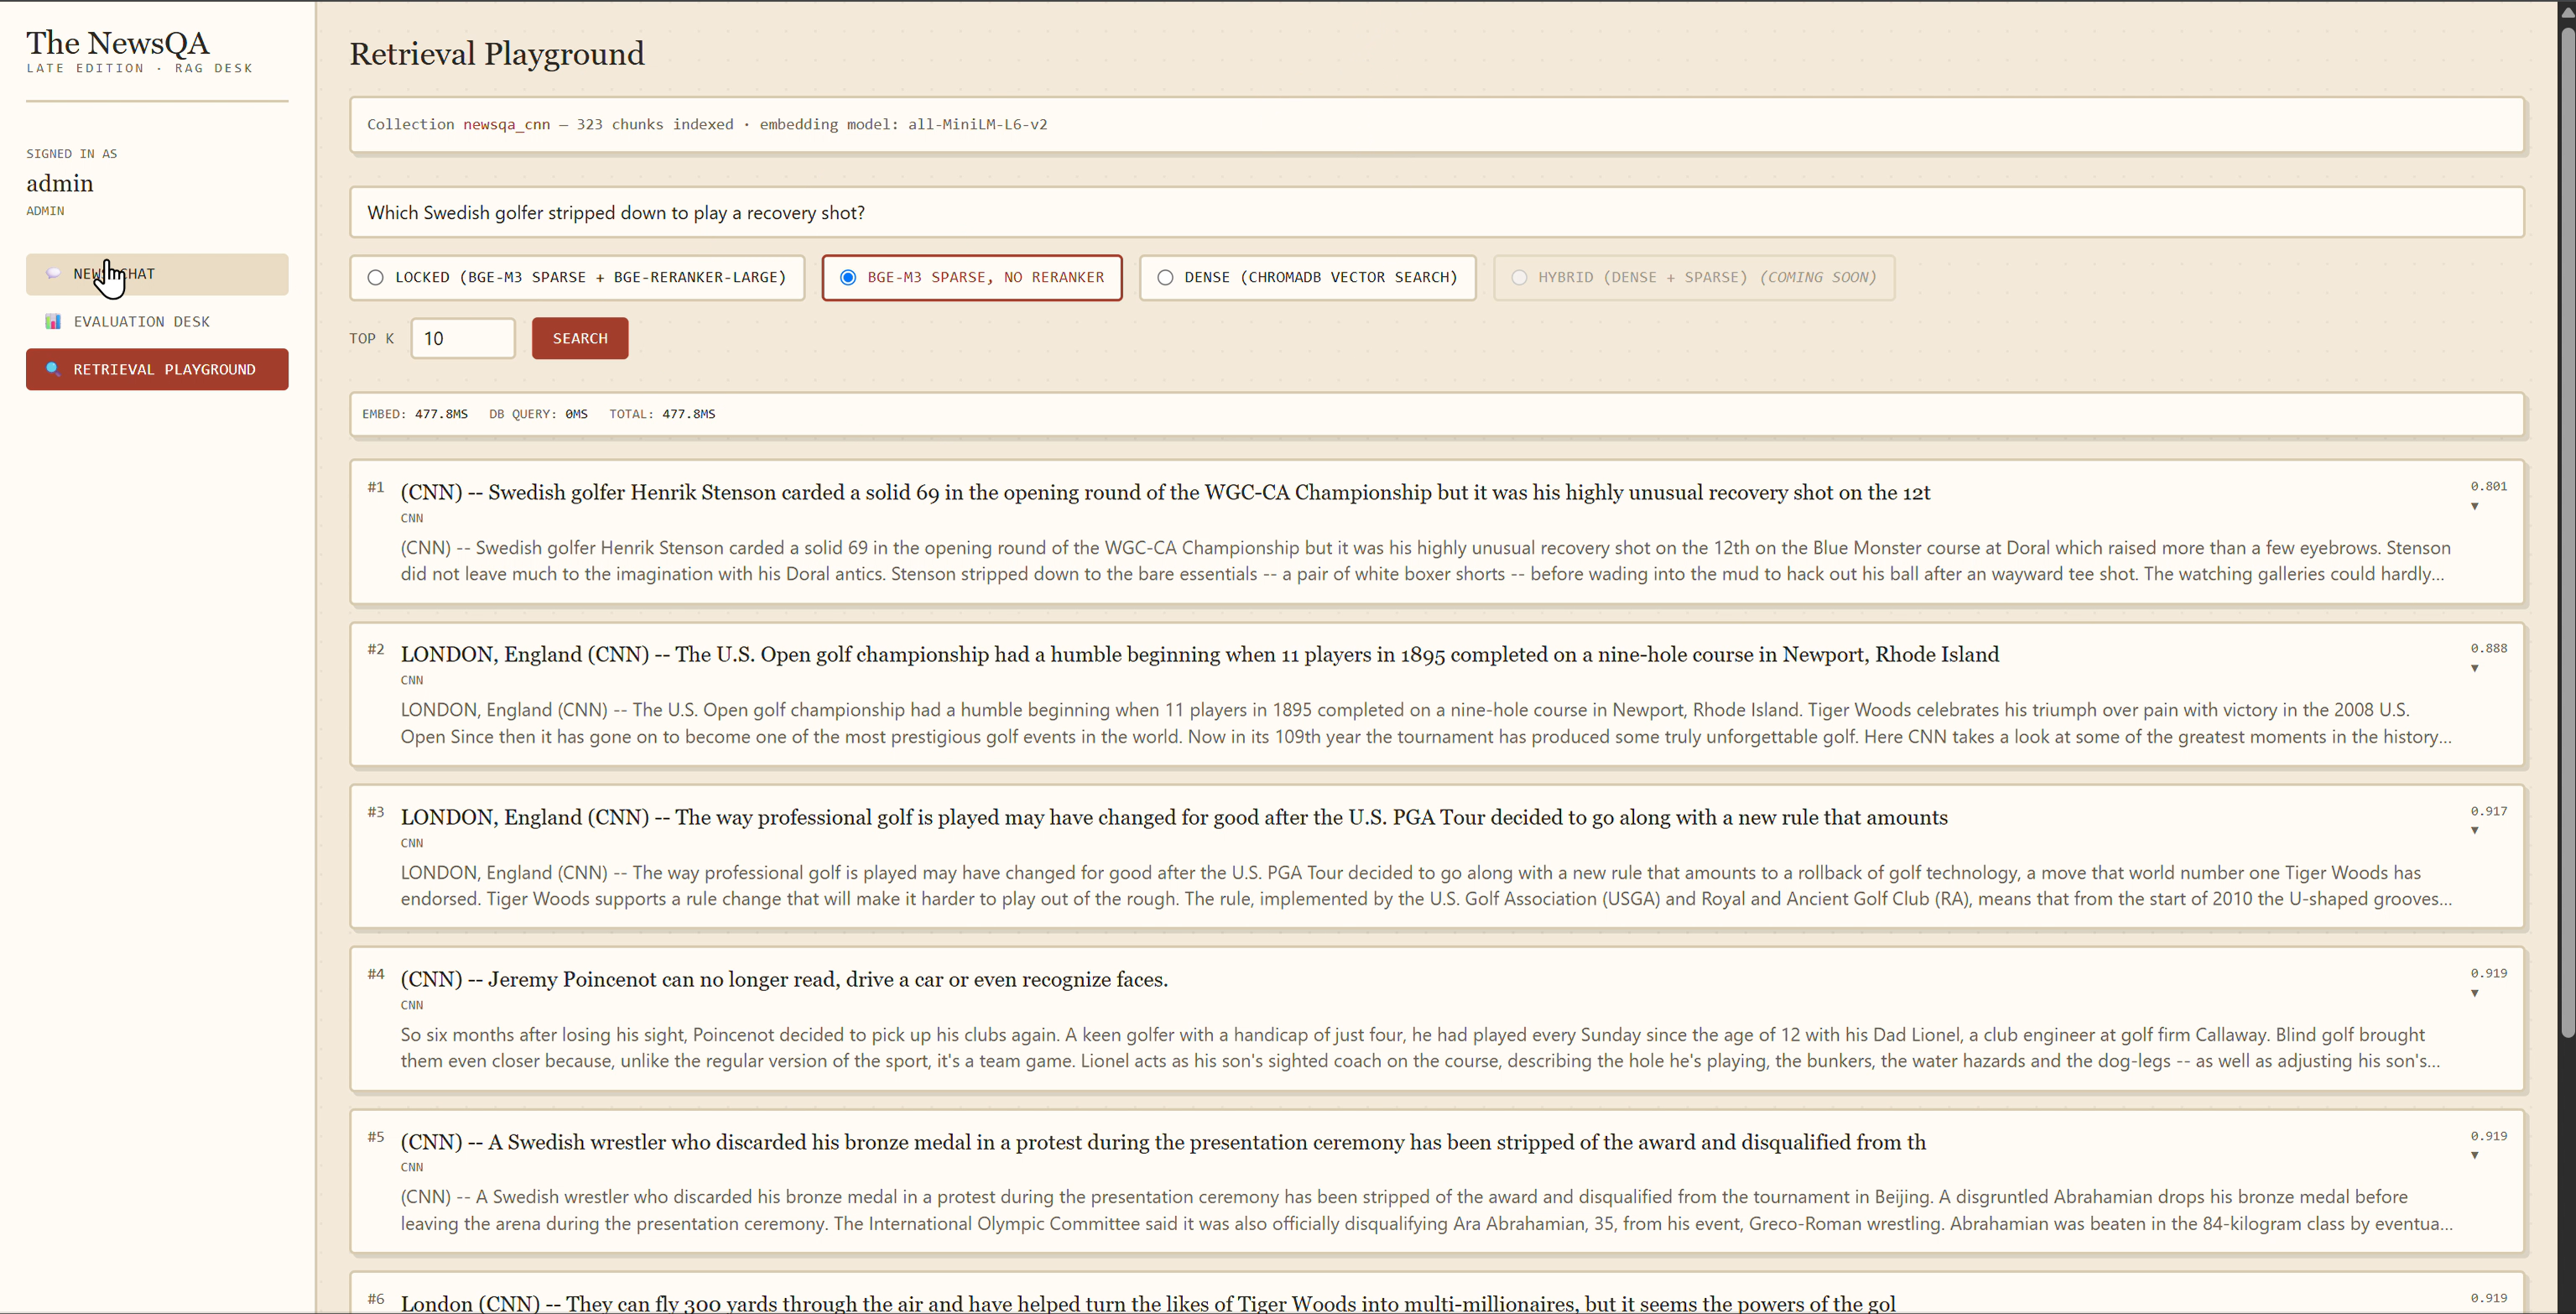
\includegraphics[width=0.92\textwidth]{../figures/retrieval_playground.png}%
  }{%
    \begin{center}
      \framebox[0.92\textwidth]{\rule{0pt}{6.5cm}\textbf{[Hình: Bàn thử nghiệm Retrieval Playground với thống kê chỉ mục và phân rã độ trễ]}}
    \end{center}
  }
  \caption{Giao diện Bàn thử nghiệm Truy xuất (Retrieval Playground): Cho phép kiểm tra trực tiếp kho chỉ mục \NumCorpusChunks{} chunks, xem điểm tương quan của các đoạn văn bản ứng viên và phân tích chi tiết độ trễ thực thi.}
  \label{fig:app-retrieval}
\end{figure}
